% KubeEdgeInfer -- research presentation (main deck, 15 slides).
%
% Compile with XeLaTeX or LuaLaTeX (fontspec is used for the Cambria/Calibri
% pairing; see the fallback note below to build with plain pdfLaTeX):
%
%     latexmk -xelatex kubeedgeinfer.tex
%
% The companion code walkthrough lives in kubeedgeinfer-code.tex and is kept
% separate on purpose -- present it only if there is time for the demo.

\documentclass[aspectratio=169,11pt]{beamer}

\usepackage{booktabs}
\usepackage{array}
\usepackage{makecell}
\renewcommand\theadfont{\bfseries}
\usepackage{tikz}
\usepackage{pgfplots}
\pgfplotsset{compat=1.18}
\usetikzlibrary{positioning,arrows.meta,shapes.geometric,calc}

% ---------------------------------------------------------------- fonts
% Fonts. Carlito and Caladea are the metric-compatible open equivalents of
% Calibri and Cambria -- the pairing the .pptx uses -- so this compiles the same
% on any machine without needing the Microsoft fonts. Two documented swaps:
%
%   * have the real fonts?  Carlito -> Calibri, Caladea -> Cambria below.
%   * no XeLaTeX/LuaLaTeX?  replace this whole block with \usepackage{lmodern}
%                           and drop \headfont (it falls back to \rmfamily).
%
% On Debian/Ubuntu the fonts come from fonts-crosextra-carlito and
% fonts-crosextra-caladea; both are also freely downloadable on macOS/Windows.
\usepackage{fontspec}
\setsansfont{Carlito}
\newfontfamily\headfont{Caladea}
\setmonofont{DejaVu Sans Mono}[Scale=0.82]
\renewcommand{\familydefault}{\sfdefault}

% ---------------------------------------------------------------- palette
\definecolor{keink}  {HTML}{141821}   % near-black slate: dark slides
\definecolor{keink2} {HTML}{232A38}   % raised surface on dark slides
\definecolor{kemist} {HTML}{F1F3F7}   % card tint on light slides
\definecolor{kemist2}{HTML}{F7F8FA}   % alternate row tint
\definecolor{keamber}{HTML}{E07B39}   % accent: thermal / novelty
\definecolor{keteal} {HTML}{1F8A80}   % accent: telemetry / healthy
\definecolor{kemuted}{HTML}{6B7280}
\definecolor{kebody} {HTML}{3E4658}

% ---------------------------------------------------------------- theme
\usetheme{default}
\usecolortheme{default}
\setbeamertemplate{navigation symbols}{}
\setbeamercolor{normal text}{fg=keink,bg=white}
\setbeamercolor{structure}{fg=keamber}
\setbeamerfont{frametitle}{size=\Large,series=\bfseries}
\setbeamercolor{frametitle}{fg=keink,bg=white}
\setbeamertemplate{frametitle}{%
  \vspace{0.35em}%
  {\usebeamerfont{framesubtitle}\scriptsize\bfseries\color{keamber}%
   \MakeUppercase{\insertframesubtitle}}\par\vspace{0.15em}%
  {\headfont\Large\bfseries\color{keink}\insertframetitle}\par\vspace{0.2em}%
}
% Footer: a page number and an optional caveat line, nothing decorative.
\newcommand{\kefoot}[1]{%
  \vfill{\scriptsize\itshape\color{kemuted}#1}%
}
\setbeamertemplate{footline}{%
  \hfill{\tiny\color{kemuted}\insertframenumber}\hspace{1.2em}\vspace{0.6em}%
}

% ---------------------------------------------------------------- helpers
% A tinted card. Used everywhere in place of bullet lists.
\newcommand{\kecard}[3][kemist]{%
  \begin{beamercolorbox}[wd=#2,sep=6pt,rounded=true]{}%
    \colorbox{#1}{\begin{minipage}{\dimexpr#2-14pt\relax}#3\end{minipage}}%
  \end{beamercolorbox}}
% A numbered marker circle -- the recurring motif of the deck.
\newcommand{\kedot}[2][keamber]{%
  \tikz[baseline=(n.base)]{\node[circle,fill=#1,text=white,inner sep=1.6pt,
    font=\scriptsize\bfseries,minimum size=1.6em] (n) {#2};}}
\newcommand{\kehead}[1]{{\bfseries\color{keink}#1}}
\newcommand{\kesub}[1]{{\footnotesize\color{kebody}#1}}
\newcommand{\kelim}[1]{{\scriptsize\itshape\color{keamber!75!black}#1}}
% Ragged-right p-column, used for every wrapping table cell.
\newcolumntype{R}[1]{>{\raggedright\arraybackslash}p{#1}}

% Dark slide background, applied per-frame.
\newcommand{\kedark}{%
  \setbeamercolor{background canvas}{bg=keink}%
  \setbeamercolor{normal text}{fg=white}%
  \usebeamercolor[fg]{normal text}}

\title{Sharing One Big AI Model Across Small Machines --- and Fixing the
       Split While It Runs}
\author{}
\institute{}
\date{}

\begin{document}

% =============================================================== 1. Title
{\kedark
\begin{frame}[plain]
  \vspace{1.2em}
  {\scriptsize\bfseries\color{keamber}\ttfamily KUBEEDGEINFER}\par\vspace{0.8em}
  {\headfont\LARGE\bfseries\color{white}
   Sharing One Big AI Model Across Small Machines\\[0.25em]
   --- and Fixing the Split While It Runs}\par\vspace{1.0em}
  {\color{keink2!30!white}\small
   Most systems choose how to cut the model once. We keep checking, and
   change the cut whenever the machines change.}\par\vspace{1.4em}
  {\footnotesize\color{keink2!45!white}
   \colorbox{keink2}{\strut\ Kernel measuring (eBPF)\ }\quad
   \colorbox{keink2}{\strut\ Kubernetes\ }\quad
   \colorbox{keink2}{\strut\ Split by layer\ }\quad
   \colorbox{keink2}{\strut\ Everyday machines\ }}\par\vspace{1.6em}
  {\small\bfseries\color{keteal}Research Presentation}\par\vspace{0.3em}
  {\footnotesize\color{kemuted}Author:\quad Institution:\quad Date:}
\end{frame}}

% =============================================================== 2. Introduction
\begin{frame}[shrink=20]
  \framesubtitle{Introduction}
  \frametitle{The machines keep changing}
  \begin{columns}[T]
  \begin{column}{0.60\textwidth}
    \kecard{\textwidth}{%
      \kedot[keteal]{1}\ \kehead{Why we split the model at all}\par\vspace{0.3em}
      \kesub{A big AI model is too large for one laptop or small PC. So we
      cut it into blocks of layers and give one block to each machine. Where we
      cut is the most important choice we make.}}\vspace{0.4em}
    \kecard{\textwidth}{%
      \kedot[keteal]{2}\ \kehead{Small machines are not like data centres}\par\vspace{0.3em}
      \kesub{Data centre servers are all the same and stay cool. Our
      machines are laptops and cheap GPU boxes on WiFi. They get hot and slow
      down, their network speed wanders, and sometimes they switch off.}}\vspace{0.4em}
    \kecard{\textwidth}{%
      \kedot{3}\ \kehead{What other systems do today}\par\vspace{0.3em}
      \kesub{They measure the machines once, pick a cut, and never look
      again. That cut is right at the start and gets more and more wrong as the
      machines change.}}
  \end{column}
  \begin{column}{0.36\textwidth}
    \colorbox{keink}{\begin{minipage}{\dimexpr\textwidth-14pt\relax}
      \vspace{0.4em}
      {\scriptsize\bfseries\color{keamber}WHAT THAT COSTS}\par\vspace{0.8em}
      {\headfont\Huge\bfseries\color{white}2.4$\times$}\par
      {\scriptsize\color{white!62!keink}slower on the busiest machine when
       one machine gets hot and the cut never changes}\par\vspace{0.9em}
      {\headfont\Huge\bfseries\color{white}4.3$\times$}\par
      {\scriptsize\color{white!62!keink}slower when a slow network and a hot
       GPU happen at the same time}\par\vspace{0.9em}
      {\headfont\Huge\bfseries\color{white}0}\par
      {\scriptsize\color{white!62!keink}answers given after one machine
       dies, if nothing is re-planned}
      \vspace{0.5em}
    \end{minipage}}
  \end{column}
  \end{columns}
  \kefoot{Numbers from the test on slide 11 (12 layers, 3 machines).}
\end{frame}

% =============================================================== 3. Lit review I
\begin{frame}[shrink=20]
  \framesubtitle{Literature review (1 of 2)}
  \frametitle{How other systems split the model}
  \footnotesize
  \begin{tabular}{@{}R{0.20\textwidth}R{0.44\textwidth}R{0.30\textwidth}@{}}
    \multicolumn{1}{@{}l}{} &
      {\scriptsize\bfseries\color{kemuted}CONTRIBUTION} &
      {\scriptsize\bfseries\color{keamber}WHAT IT DOES NOT DO}\\
    \midrule
    \kehead{EdgeShard}\newline
      {\scriptsize\color{keteal}\bfseries IEEE IoT-J, 2024}\newline
      {\tiny\ttfamily arXiv:2405.14371} &
      \kesub{Picks which devices to use and where to cut, with an exact
      solver. Up to 50\% less delay and 2$\times$ more work done, tested on 15
      real devices.} &
      \kelim{Measures the devices once, before running. The plan never changes
      after that.}\\[0.5em]
    \kehead{Galaxy}\newline
      {\scriptsize\color{keteal}\bfseries IEEE INFOCOM, 2024}\newline
      {\tiny\ttfamily arXiv:2405.17245} &
      \kesub{Splits the work inside each layer instead of by layer, and
      overlaps computing with sending. Up to 2.5$\times$ less delay.} &
      \kelim{The plan is made once, before running. Nothing is re-planned while
      it runs.}\\[0.5em]
    \kehead{Helix}\newline
      {\scriptsize\color{keteal}\bfseries ACM ASPLOS, 2025}\newline
      {\tiny\ttfamily arXiv:2406.01566} &
      \kesub{Treats serving on mixed GPUs as a flow problem, and chooses
      placement and routing together. Up to 3.3$\times$ more work done on
      24--42 machines.} &
      \kelim{Built for data centre GPUs. Its solver is far too slow to re-run
      every few seconds.}\\[0.5em]
    \kehead{TPI-LLM}\newline
      {\scriptsize\color{keteal}\bfseries arXiv, 2024}\newline
      {\tiny\ttfamily arXiv:2410.00531} &
      \kesub{Argues that splitting inside layers beats splitting by layer on
      small devices. Clever memory handling lets 70B models run in small RAM.} &
      \kelim{Improves memory use, but does not react when a machine slows
      down.}\\[0.5em]
    \kehead{prima.cpp}\newline
      {\scriptsize\color{keteal}\bfseries arXiv, 2025}\newline
      {\tiny\ttfamily arXiv:2504.08791} &
      \kesub{Runs 30--70B models on real home machines. Shares work between
      CPU and GPU and hides slow disk reads. 5--17$\times$ faster per word than
      llama.cpp.} &
      \kelim{Decides the plan when loading, from fixed device specs.}\\
    \bottomrule
  \end{tabular}
  \kefoot{All ten papers are from 2024--2025. Full list on slide 15.}
\end{frame}

% =============================================================== 4. Lit review II
\begin{frame}[shrink=20]
  \framesubtitle{Literature review (2 of 2)}
  \frametitle{Adapting, sharing out, and eBPF as a control tool}
  \footnotesize
  \begin{tabular}{@{}R{0.20\textwidth}R{0.44\textwidth}R{0.30\textwidth}@{}}
    \multicolumn{1}{@{}l}{} &
      {\scriptsize\bfseries\color{kemuted}CONTRIBUTION} &
      {\scriptsize\bfseries\color{keamber}WHAT IT DOES NOT DO}\\
    \midrule
    \kehead{LLM Partitioning at the Edge}\newline
      {\scriptsize\color{keteal}\bfseries arXiv, 2025}\newline
      {\tiny\ttfamily arXiv:2505.02533} &
      \kesub{Cuts the model into much smaller pieces (single attention heads)
      and moves them when memory runs low. Within 15--20\% of the best possible
      answer.} &
      \kelim{Only reacts to memory running low -- not to heat or to a slow
      network.}\\[0.5em]
    \kehead{Parallax}\newline
      {\scriptsize\color{keteal}\bfseries arXiv, 2025}\newline
      {\tiny\ttfamily arXiv:2509.26182} &
      \kesub{Serves a model across a pool of volunteer machines of all
      shapes, with no central cluster in charge.} &
      \kelim{Spreads the work out well, but measures nothing inside the
      kernel.}\\[0.5em]
    \kehead{Adaptive Layer Splitting (MBRL)}\newline
      {\scriptsize\color{keteal}\bfseries FITEE, Springer, 2025}\newline
      {\tiny\ttfamily doi:10.1631/FITEE.2400468} &
      \kesub{Learns where to cut, and moves the cut as the wireless signal
      changes. It does keep adapting, which is rare.} &
      \kelim{The policy must be trained first, and cannot promise the best
      answer. Only one cut point.}\\[0.5em]
    \kehead{Distributed LLMs \& MLLMs Survey}\newline
      {\scriptsize\color{keteal}\bfseries arXiv, 2025}\newline
      {\tiny\ttfamily arXiv:2503.16585} &
      \kesub{Reviews the whole field, and lists ``adapting to machines that
      keep changing'' as an open problem.} &
      \kelim{Confirms the gap we are filling. It does not fill it.}\\[0.5em]
    \kehead{Agentic OS / sched\_ext}\newline
      {\scriptsize\color{keteal}\bfseries arXiv, 2025}\newline
      {\tiny\ttfamily arXiv:2509.01245} &
      \kesub{Loads custom Linux schedulers as eBPF programs while the system
      runs. Shows eBPF is now used to control things, not only to watch
      them.} &
      \kelim{Works on one machine's CPU tasks. Nothing about splitting a model
      across machines.}\\
    \bottomrule
  \end{tabular}
  \kefoot{All ten papers are from 2024--2025. Full list on slide 15.}
\end{frame}

% =============================================================== 5. Gap
\begin{frame}[shrink=20]
  \framesubtitle{What is missing}
  \frametitle{What past work is missing}
  \scriptsize
  % Every cell is a \makecell[tl] over `l' columns rather than a p-column: a
  % p-column whose neighbours wrap drifts out of row alignment, and manual
  % breaks keep all five columns on one baseline.
  \setcellgapes{3.5pt}\makegapedcells
  \begin{tabular}{@{}lllll@{}}
    \toprule
    \thead[tl]{Capability} &
    \thead[tl]{Data centre\\serving\\(Helix)} &
    \thead[tl]{Splitting on small\\devices (EdgeShard,\\Galaxy, prima.cpp)} &
    \thead[tl]{Learned splitting\\(MBRL, head-level)} &
    \thead[tl]{\color{keamber}KubeEdgeInfer}\\
    \midrule
    \makecell[tl]{Handles machines of\\different speed} & yes & yes & yes &
      \makecell[tl]{\bfseries\color{keteal}yes}\\
    Finds the best cut for the moment & \makecell[tl]{yes, heavy\\solver} & yes &
      \makecell[tl]{no (learned or\\rule of thumb)} &
      \makecell[tl]{\bfseries\color{keteal}yes, checked\\
                    \bfseries\color{keteal}against brute force}\\
    Changes the cut while running &
      \makecell[tl]{only where\\requests go} & no & yes &
      \makecell[tl]{\bfseries\color{keteal}yes, every 2 seconds}\\
    Measures the network in the kernel & no & app-level timers &
      signal estimate &
      \makecell[tl]{\bfseries\color{keteal}yes, reads TCP\\
                    \bfseries\color{keteal}directly}\\
    Knows when a machine gets hot & no & no & no &
      \makecell[tl]{\bfseries\color{keteal}yes, reads GPU\\
                    \bfseries\color{keteal}and CPU heat}\\
    Survives a machine dying & by keeping copies & no & no &
      \makecell[tl]{\bfseries\color{keteal}yes, re-cuts in\\
                    \bfseries\color{keteal}3 seconds}\\
    Changes without restarting & not applicable & no & no &
      \makecell[tl]{\bfseries\color{keteal}yes, moves\\
                    \bfseries\color{keteal}layers live}\\
    \bottomrule
  \end{tabular}
  \kefoot{No earlier system measures the machines in the kernel and feeds
          that straight back into the cut, while the model is still
          answering.}
\end{frame}

% =============================================================== 6. Problem
{\kedark
\begin{frame}[shrink=20]
  \vspace{0.6em}
  {\scriptsize\bfseries\color{keamber}THE PROBLEM}\par\vspace{0.7em}
  {\headfont\large\color{white}
   We have $N$ model layers and $K$ machines of different speeds. While the
   model is answering, their speed, their network delay, and whether they are
   even alive all keep changing. Keep choosing a cut that makes the slowest
   machine as fast as possible --- and never restart anything to do it.}\par\vspace{1.2em}
  \begin{columns}[T]
  \begin{column}{0.62\textwidth}\footnotesize
    \kedot{1}\ {\bfseries\color{white}Measure}\par
    {\scriptsize\color{white!60!keink}Measure network delay and machine heat
     cheaply, without changing the model code.}\par\vspace{0.6em}
    \kedot[keteal]{2}\ {\bfseries\color{white}Decide}\par
    {\scriptsize\color{white!60!keink}Work out the best cut fast enough to
     redo it often, without flip-flopping when a reading is just noisy.}\par\vspace{0.6em}
    \kedot{3}\ {\bfseries\color{white}Act}\par
    {\scriptsize\color{white!60!keink}Move layers between running machines
     without losing requests or restarting anything.}\par\vspace{0.6em}
    \kedot[keteal]{4}\ {\bfseries\color{white}Heal}\par
    {\scriptsize\color{white!60!keink}Notice when a machine dies and share
     its layers among the machines that are left.}
  \end{column}
  \begin{column}{0.34\textwidth}
    \colorbox{keink2}{\begin{minipage}{\dimexpr\textwidth-14pt\relax}
      \vspace{0.4em}
      {\scriptsize\bfseries\color{keamber}THE RULES WE SET OURSELVES}\par\vspace{0.6em}
      {\footnotesize\color{white!78!keink}Ordinary Linux only.\par\vspace{0.5em}
       No special data centre network, no vendor software, no changes to the
       model code, and no assuming a machine stays alive.}
      \vspace{0.5em}
    \end{minipage}}
  \end{column}
  \end{columns}
\end{frame}}

% =============================================================== 7. Contributions
\begin{frame}[shrink=20]
  \framesubtitle{What is new}
  \frametitle{What is new in our work}
  \footnotesize
  \begin{columns}[T]
  \begin{column}{0.48\textwidth}
    \kecard{\textwidth}{\kedot{1}\ \kehead{We measure the network inside the kernel}\par
      \vspace{0.25em}\kesub{Small eBPF programs read the round-trip time Linux already
      tracks for every connection, and we feed that straight into the cut
      decision. Other systems guess with app-level timers, or use readings
      taken before the run.}}\vspace{0.35em}
    \kecard{\textwidth}{\kedot{2}\ \kehead{We never stop deciding}\par
      \vspace{0.25em}\kesub{Watch, decide, act, heal --- every 2 seconds, for as long as
      the system runs. The cut is something we keep adjusting, not a setting we
      pick once.}}\vspace{0.35em}
    \kecard{\textwidth}{\kedot{3}\ \kehead{We add brakes so it does not flip-flop}\par
      \vspace{0.25em}\kesub{The solver gives the exact best cut every time. We only apply
      a new one if it is at least 15\% better and 30 seconds have passed. The
      same brake handles heat, network and machine failure.}}
  \end{column}
  \begin{column}{0.48\textwidth}
    \kecard[kemist2]{\textwidth}{\kedot[keteal]{4}\ \kehead{We move layers without a restart}\par
      \vspace{0.25em}\kesub{Layers move between machines while requests are still in
      flight. Each plan carries a version number, machines refuse messages from
      an old plan, and because machines keep no state we can simply replay the
      request.}}\vspace{0.35em}
    \kecard[kemist2]{\textwidth}{\kedot[keteal]{5}\ \kehead{We show the gain comes from live measuring}\par
      \vspace{0.25em}\kesub{We built a ``measure once'' mode that uses the same solver
      and the same code, but freezes what it measured. So the improvement we
      report comes from measuring all the time, not from a better solver.}}\vspace{0.35em}
    \colorbox{keink}{\begin{minipage}{\dimexpr\textwidth-14pt\relax}
      \vspace{0.3em}
      {\scriptsize\bfseries\color{keamber}THE MAIN NEW IDEA}\par\vspace{0.4em}
      {\footnotesize\color{white!80!keink}We did not invent a new splitting
       algorithm. We took the standard one and put it inside a loop that keeps
       measuring the real machines and never stops.}
      \vspace{0.3em}
    \end{minipage}}
  \end{column}
  \end{columns}
  \kefoot{Items 1--3 are the main new ideas.}
\end{frame}

% =============================================================== 8. Architecture
\begin{frame}[shrink=20]
  \framesubtitle{Our system}
  \frametitle{How the loop works}
  \centering
  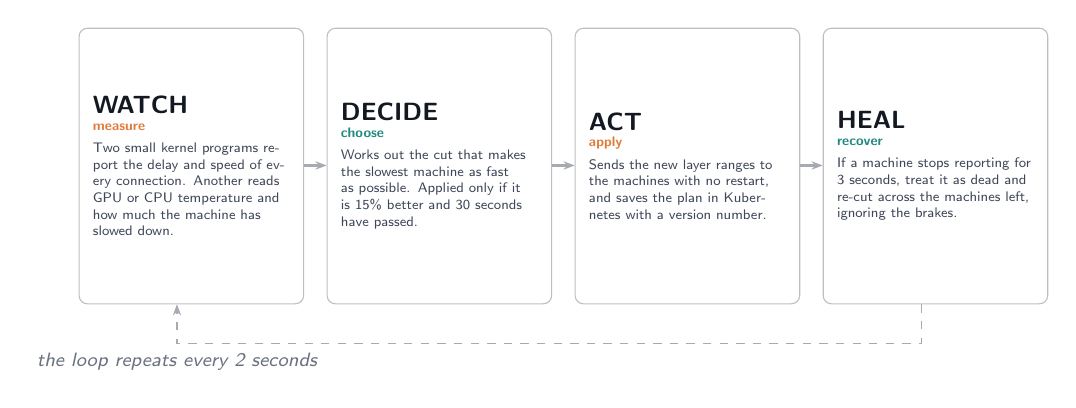
\begin{tikzpicture}[
      % Four stages laid out across the 12.8cm text block: 2.85cm-wide cards on
      % a 3.15cm pitch, so the row fits without a \resizebox shrinking the text.
      stage/.style={draw=kemuted!45,fill=white,rounded corners=3pt,
                    text width=2.5cm,align=left,inner sep=5pt,
                    minimum height=3.5cm,anchor=north west},
      font=\tiny]
    \node[stage] (w) at (0,0) {%
      {\small\headfont\bfseries\color{keink}WATCH}\\
      {\tiny\bfseries\color{keamber}measure}\\[0.4em]
      \color{kebody}Two small kernel programs report the delay and speed of
      every connection. Another reads GPU or CPU temperature and how much the
      machine has slowed down.};
    \node[stage] (d) at (3.15,0) {%
      {\small\headfont\bfseries\color{keink}DECIDE}\\
      {\tiny\bfseries\color{keteal}choose}\\[0.4em]
      \color{kebody}Works out the cut that makes the slowest machine as fast
      as possible. Applied only if it is 15\% better and 30 seconds have
      passed.};
    \node[stage] (a) at (6.3,0) {%
      {\small\headfont\bfseries\color{keink}ACT}\\
      {\tiny\bfseries\color{keamber}apply}\\[0.4em]
      \color{kebody}Sends the new layer ranges to the machines with no
      restart, and saves the plan in Kubernetes with a version number.};
    \node[stage] (h) at (9.45,0) {%
      {\small\headfont\bfseries\color{keink}HEAL}\\
      {\tiny\bfseries\color{keteal}recover}\\[0.4em]
      \color{kebody}If a machine stops reporting for 3 seconds, treat it as
      dead and re-cut across the machines left, ignoring the brakes.};
    \foreach \a/\b in {w/d,d/a,a/h}
      \draw[-{Stealth[length=4pt]},kemuted!60,thick]
        ($(\a.north east)+(0,-1.75cm)$) -- ($(\b.north west)+(0,-1.75cm)$);
    % The return edge: what the one-shot systems in the literature do not have.
    \draw[-{Stealth[length=4pt]},kemuted!60,dashed]
      ($(h.south west)+(1.25cm,0)$) -- ++(0,-0.5cm)
      -| ($(w.south west)+(1.25cm,0)$)
      node[pos=0.5,below,font=\scriptsize\itshape,color=kemuted]
      {the loop repeats every 2 seconds};
  \end{tikzpicture}
  \par\vspace{0.6em}
  \kecard{\textwidth}{\kesub{\textbf{Staying correct:} every plan carries a
    version number. Machines refuse messages from an old plan. The router then
    fetches the new plan and replays the request from the start. Machines keep
    no state, so replaying is always safe.}}
\end{frame}

% =============================================================== 9. Formulation
\begin{frame}[shrink=20]
  \framesubtitle{Our system}
  \frametitle{The maths, and how we keep it steady}
  \begin{columns}[T]
  \begin{column}{0.47\textwidth}\footnotesize
    \kecard{\textwidth}{%
      {\bfseries\color{keamber}The goal}\par\vspace{0.4em}
      \begin{center}\bfseries make the slowest machine as fast as possible
      \end{center}
      \vspace{-0.4em}
      \[\text{machine time}=\frac{\text{layers}\times\text{time per layer}}
                                 {\text{speed}} + \text{network delay}\]
      \vspace{-0.4em}
      \kesub{Each machine gets a block of layers next to each other, and
      together they cover all $N$ layers. A machine given zero layers costs
      nothing at all --- so the solver can skip a machine whose network has
      become too slow to be worth using.}}\vspace{0.4em}
    \kecard{\textwidth}{%
      {\bfseries\color{keteal}How we solve it}\par\vspace{0.4em}
      \[\mathit{best}[j][w]=\text{the best we can do for the first }j
        \text{ layers on }w\text{ machines}\]
      \vspace{-0.4em}
      \kesub{This is a classic problem with a known exact answer. For 12 layers
      and 3 machines it takes about 1{,}700 steps, so redoing it every 2
      seconds costs nothing. We checked it against brute force on 200 random
      cases.}}
  \end{column}
  \begin{column}{0.49\textwidth}
    \colorbox{keink}{\begin{minipage}{\dimexpr\textwidth-14pt\relax}\footnotesize
      \vspace{0.4em}
      {\bfseries\color{keamber}Why a solver alone is not enough}\par
      \vspace{0.4em}
      {\scriptsize\color{white!68!keink}Measurements jump around. If we
       applied the best answer every 2 seconds, the system would keep moving
       layers for tiny gains. Three rules fix that:}\par\vspace{0.8em}
      {\color{white}\bfseries\scriptsize\textcolor{keteal}{$\bullet$}\ Must be clearly better}\par
      {\scriptsize\color{white!60!keink}Only change if the new cut beats the
       current one, measured right now, by 15\%.}\par\vspace{0.5em}
      {\color{white}\bfseries\scriptsize\textcolor{keteal}{$\bullet$}\ Wait between changes}\par
      {\scriptsize\color{white!60!keink}At most one change every 30 seconds,
       so a short spike cannot start a wobble.}\par\vspace{0.5em}
      {\color{white}\bfseries\scriptsize\textcolor{keamber}{$\bullet$}\ Except when a machine dies}\par
      {\scriptsize\color{white!60!keink}If the set of machines changes,
       ignore both rules and re-cut at once. Being correct matters more than
       being steady.}\par\vspace{0.8em}
      {\tiny\itshape\color{white!52!keink}Both numbers can be changed while
       the system is running.}
      \vspace{0.4em}
    \end{minipage}}
  \end{column}
  \end{columns}
\end{frame}

% =============================================================== 10. Implementation
\begin{frame}[shrink=20]
  \framesubtitle{Our system}
  \frametitle{What we built}
  \begin{columns}[T]
  \begin{column}{0.58\textwidth}\footnotesize
    \kecard{\textwidth}{\textcolor{keamber}{$\bullet$}\ \kehead{Agent on each machine}
      {\tiny\ttfamily\color{kemuted}Go and C}\par\vspace{0.2em}
      \kesub{Runs on every machine with kernel access. Loads the eBPF programs,
      watches only the ports we care about, and reports network delay plus GPU
      state. GPU readings can be simulated, taken from CPU heat sensors, or read
      from a real NVIDIA card.}}\vspace{0.3em}
    \kecard[kemist2]{\textwidth}{\textcolor{keteal}{$\bullet$}\ \kehead{Central controller}
      {\tiny\ttfamily\color{kemuted}Go}\par\vspace{0.2em}
      \kesub{Collects all the readings, runs the decider, saves the plan in
      Kubernetes and sends it to the machines. A watchdog forces a re-cut if a
      machine goes quiet for 3 seconds.}}\vspace{0.3em}
    \kecard{\textwidth}{\textcolor{keamber}{$\bullet$}\ \kehead{Workers and router}
      {\tiny\ttfamily\color{kemuted}Python}\par\vspace{0.2em}
      \kesub{Each worker holds a block of layers and keeps no state. Two
      backends: a fake one for testing, and real GPT-2. Runs on CPU or GPU. The
      router sends each request through the machines in order.}}\vspace{0.3em}
    \kecard[kemist2]{\textwidth}{\textcolor{keteal}{$\bullet$}\ \kehead{Test harness}
      {\tiny\ttfamily\color{kemuted}Python}\par\vspace{0.2em}
      \kesub{Five fault situations $\times$ three modes. Measures idle time,
      words per second, and time to the first word. Also tries different brake
      settings.}}
  \end{column}
  \begin{column}{0.38\textwidth}
    \colorbox{keink}{\begin{minipage}{\dimexpr\textwidth-14pt\relax}
      \vspace{0.4em}
      {\footnotesize\bfseries\color{keamber}What is real, what is not}\par\vspace{0.6em}
      {\scriptsize\color{white!62!keink}
       \textcolor{keteal}{$\bullet$}\ The eBPF part is real, not simulated.
       It is built against the running kernel and loaded into
       it.\par\vspace{0.45em}
       \textcolor{keteal}{$\bullet$}\ On a single test host you get real eBPF,
       but a fake network and a fake GPU.\par\vspace{0.45em}
       \textcolor{keteal}{$\bullet$}\ Our scripts turn a few laptops and GPU
       boxes on the same network into one cluster, with no config
       editing.\par\vspace{0.45em}
       \textcolor{keteal}{$\bullet$}\ Real NVIDIA readings on GPU machines; real
       CPU heat readings on laptops with no GPU.\par\vspace{0.45em}
       \textcolor{keteal}{$\bullet$}\ The split-up GPT-2 gives exactly the same
       text as running it on one machine.}
      \vspace{0.5em}
    \end{minipage}}
  \end{column}
  \end{columns}
\end{frame}

% =============================================================== 11. Results chart
\begin{frame}[shrink=20]
  \framesubtitle{Results}
  \frametitle{How slow the busiest machine gets}
  \begin{columns}[T]
  \begin{column}{0.62\textwidth}
    \centering
    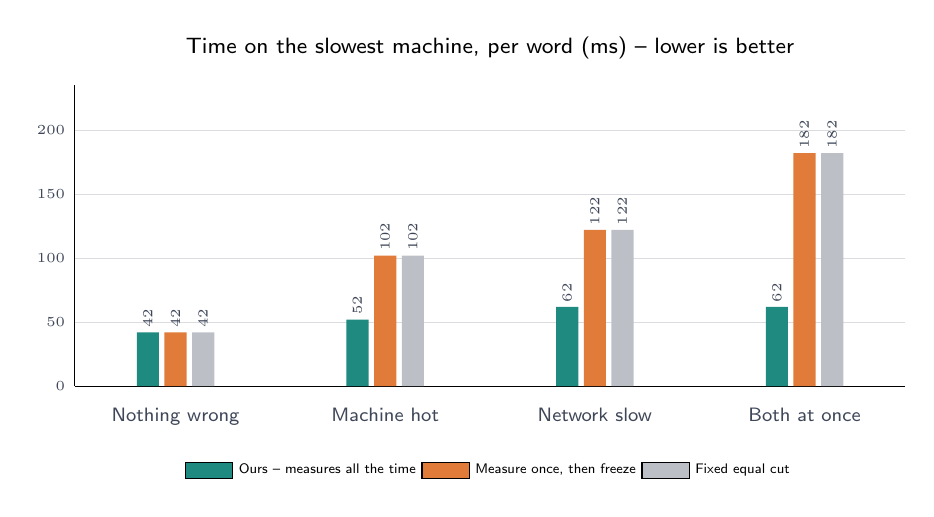
\begin{tikzpicture}
      \begin{axis}[
        width=\textwidth, height=5.4cm,
        ybar, bar width=8pt, enlarge x limits=0.16,
        ymin=0, ymax=235, ytick={0,50,100,150,200},
        ylabel={}, title={\footnotesize Time on the slowest machine, per word (ms) -- lower is better},
        symbolic x coords={{Nothing wrong},{Machine hot},{Network slow},{Both at once}},
        xtick=data, xticklabel style={font=\scriptsize,color=kebody},
        yticklabel style={font=\tiny,color=kebody},
        ymajorgrids, grid style={kemuted!25},
        axis lines*=left, tick style={draw=none},
        nodes near coords, area legend,
        every node near coord/.append style=
          {font=\tiny,color=kebody,rotate=90,anchor=west,inner sep=1.5pt},
        legend style={at={(0.5,-0.22)},anchor=north,legend columns=3,
                      draw=none,font=\tiny},
        ]
        \addplot[fill=keteal,draw=none]  coordinates
          {({Nothing wrong},42) ({Machine hot},52)
           ({Network slow},62) ({Both at once},62)};
        \addplot[fill=keamber,draw=none] coordinates
          {({Nothing wrong},42) ({Machine hot},102)
           ({Network slow},122) ({Both at once},182)};
        \addplot[fill=kemuted!45,draw=none] coordinates
          {({Nothing wrong},42) ({Machine hot},102)
           ({Network slow},122) ({Both at once},182)};
        \legend{Ours -- measures all the time,
                Measure once{,} then freeze,
                Fixed equal cut}
      \end{axis}
    \end{tikzpicture}
  \end{column}
  \begin{column}{0.34\textwidth}\footnotesize
    \kecard{\textwidth}{{\headfont\huge\bfseries\color{keteal}49\%}\quad
      \kesub{better than both when a machine gets hot}}\vspace{0.35em}
    \kecard{\textwidth}{{\headfont\huge\bfseries\color{keteal}49\%}\quad
      \kesub{better than both when the network slows}}\vspace{0.35em}
    \colorbox{keink}{\begin{minipage}{\dimexpr\textwidth-14pt\relax}
      \vspace{0.2em}{\headfont\huge\bfseries\color{keamber}66\%}\par
      {\scriptsize\color{white!62!keink}better than both when both happen at
       once}\vspace{0.2em}\end{minipage}}\vspace{0.35em}
    \kecard[keamber!12!white]{\textwidth}{{\scriptsize\color{keamber!60!black}
      When a machine dies, the fixed cut has no plan for the machines left,
      so everything stops. Ours re-cuts and keeps going at 62\,ms.}}
  \end{column}
  \end{columns}
  \kefoot{Measured with \texttt{bench/dpsim}: 12 layers, 3 machines,
          10\,ms per layer, one machine slowed to 0.4$\times$, 80\,ms network
          delay.}
\end{frame}

% =============================================================== 12. Results behaviour
\begin{frame}[shrink=20]
  \framesubtitle{Results}
  \frametitle{What the solver actually decides}
  \begin{columns}[T]
  \begin{column}{0.58\textwidth}\footnotesize
    \setcellgapes{4pt}\makegapedcells
    \begin{tabular}{@{}llr@{}}
      & {\tiny\color{kemuted}layers given to machine 1 / 2 / 3} & \\
      \midrule
      \makecell[tl]{\bfseries\color{keink}All machines healthy\\
        {\tiny\ttfamily\color{kemuted}3 machines, all fine}} &
        {\ttfamily\scriptsize 0-4\ \ 4-8\ \ 8-12} &
        {\headfont\color{keteal}\bfseries 42\,ms}\\
      \makecell[tl]{\bfseries\color{keink}Machine 2 gets hot\\
        {\tiny\ttfamily\color{kemuted}speed drops to 0.4x}} &
        {\ttfamily\scriptsize 0-5\ \ 5-7\ \ 7-12} &
        {\headfont\color{keamber}\bfseries 52\,ms}\\
      \makecell[tl]{\bfseries\color{keink}Network to machine 2 slows\\
        {\tiny\ttfamily\color{kemuted}delay 2 ms -> 82 ms}} &
        {\ttfamily\scriptsize 0-6\ \ \textcolor{kemuted}{empty}\ \ 6-12} &
        {\headfont\color{keamber}\bfseries 62\,ms}\\
      \makecell[tl]{\bfseries\color{keink}Machine 3 dies\\
        {\tiny\ttfamily\color{kemuted}3 machines -> 2}} &
        {\ttfamily\scriptsize 0-6\ \ 6-12} &
        {\headfont\color{keamber}\bfseries 62\,ms}\\
      \bottomrule
    \end{tabular}
  \end{column}
  \begin{column}{0.38\textwidth}
    \colorbox{keink}{\begin{minipage}{\dimexpr\textwidth-14pt\relax}
      \vspace{0.3em}
      {\footnotesize\bfseries\color{keamber}It can skip a machine}\par\vspace{0.4em}
      {\scriptsize\color{white!65!keink}When the network to machine 2 slows
       to 80\,ms, the solver gives it zero layers. A machine with no layers
       costs nothing at all, so the router skips it and the other two take all
       12 layers. Nobody told it to do this --- it falls out of the maths.}
      \vspace{0.3em}
    \end{minipage}}\par\vspace{0.5em}
    {\scriptsize
     \textcolor{keteal}{$\bullet$}\ \kehead{It finds the best answer}\par
     {\tiny\color{kebody}The solver matched brute force on 200 random test
      cases.}\par\vspace{0.4em}
     \textcolor{keteal}{$\bullet$}\ \kehead{It gives the same answers}\par
     {\tiny\color{kebody}GPT-2 split over 3 machines produces exactly the same
      text as one machine.}\par\vspace{0.4em}
     \textcolor{keteal}{$\bullet$}\ \kehead{How good the estimate is}\par
     {\tiny\color{kebody}Our predicted time is always about 3$\times$ lower than
      the real time. Good for ranking cuts, not for predicting real speed.}}
  \end{column}
  \end{columns}
  \kefoot{Words per second, time to the first word, and real idle time come
          from \texttt{bench/run.py}, which needs a running cluster.}
\end{frame}

% =============================================================== 13. Comparison
\begin{frame}[shrink=20]
  \framesubtitle{Comparison}
  \frametitle{How we compare with the closest systems}
  \scriptsize
  \setcellgapes{3.5pt}\makegapedcells
  \begin{tabular}{@{}llllll@{}}
    \toprule
    &
    \thead[tl]{EdgeShard\\(IoT-J 24)} &
    \thead[tl]{Galaxy\\(INFOCOM 24)} &
    \thead[tl]{Helix\\(ASPLOS 25)} &
    \thead[tl]{prima.cpp\\(2025)} &
    \thead[tl]{\color{keamber}KubeEdgeInfer}\\
    \midrule
    How the model is split & by layer & \makecell[tl]{inside\\layers} &
      \makecell[tl]{by layer +\\routing} & ring of layers &
      \makecell[tl]{\bfseries\color{keteal}by layer}\\
    How the cut is chosen & exact solver & \makecell[tl]{rule of\\thumb} &
      \makecell[tl]{heavy\\solver} & custom scheduler &
      \makecell[tl]{\bfseries\color{keteal}exact solver}\\
    Where its numbers come from & measured before & measured before &
      measured before & device specs &
      \makecell[tl]{\bfseries\color{keteal}kernel + GPU, live}\\
    Re-cuts while running & no & no & only routing & no &
      \makecell[tl]{\bfseries\color{keteal}every 2 seconds}\\
    Reacts to machines getting hot & no & no & no & no &
      \makecell[tl]{\bfseries\color{keteal}yes}\\
    Survives a machine dying & no & no & by keeping copies & no &
      \makecell[tl]{\bfseries\color{keteal}yes, within 3 seconds}\\
    What it runs on & \makecell[tl]{15 small\\devices} & small devices &
      \makecell[tl]{24--42 GPU\\servers} & home machines &
      \makecell[tl]{\bfseries\color{keteal}laptops + GPU boxes}\\
    Improvement they report & 50\% less delay &
      \makecell[tl]{2.5$\times$ less\\delay} &
      \makecell[tl]{3.3$\times$ more\\work} &
      \makecell[tl]{5--17$\times$ faster\\words} &
      \makecell[tl]{\bfseries\color{keteal}49--66\% better*}\\
    \bottomrule
  \end{tabular}
  \kefoot{* We measure how slow the busiest machine gets, against a fixed cut
          and a measure-once version of our own system. That is not the same
          measurement as the other columns.}
\end{frame}

% =============================================================== 14. Conclusion
{\kedark
\begin{frame}[shrink=20]
  \vspace{0.5em}
  {\scriptsize\bfseries\color{keamber}CONCLUSION}\par\vspace{0.7em}
  {\headfont\Large\bfseries\color{white}
   Where to cut the model is a decision you should keep making, not one you
   make once.}\par\vspace{0.9em}
  {\footnotesize\color{white!62!keink}
   We keep a standard, exact solver running all the time. It is fed by
   network delays read from the kernel and by real temperature readings, and it
   moves layers on a live system with no restart. On a set of ordinary machines,
   that is the difference between a plan that was right once and a plan that
   stays right.}\par\vspace{1.1em}
  \begin{columns}[T]
  \begin{column}{0.60\textwidth}\footnotesize
    \kedot{1}\ {\bfseries\color{white}The exact answer is cheap}\par
    {\scriptsize\color{white!58!keink}Working out the best cut takes
     microseconds. There is no reason to do it only once.}\par\vspace{0.5em}
    \kedot[keteal]{2}\ {\bfseries\color{white}The brakes are what make it usable}\par
    {\scriptsize\color{white!58!keink}One ``must be clearly better'' rule and
     one ``wait a bit'' rule handle heat, network and machine failure all the
     same way.}\par\vspace{0.5em}
    \kedot[keteal]{3}\ {\bfseries\color{white}Kernel measuring is free}\par
    {\scriptsize\color{white!58!keink}eBPF sees what really went over the
     network, not what the program thinks it sent.}
  \end{column}
  \begin{column}{0.36\textwidth}
    \colorbox{keink2}{\begin{minipage}{\dimexpr\textwidth-14pt\relax}
      \vspace{0.3em}
      {\footnotesize\bfseries\color{keamber}Next steps}\par\vspace{0.5em}
      {\scriptsize\color{white!62!keink}
       \textcolor{keteal}{$\bullet$}\ Support a Llama-size model, so two
       8\,GB cards can hold a real modern model between
       them.\par\vspace{0.4em}
       \textcolor{keteal}{$\bullet$}\ Run heavy load for a long time, to see a
       GPU really slow down instead of flat lines.\par\vspace{0.4em}
       \textcolor{keteal}{$\bullet$}\ Allow cuts that are not one solid block
       per machine, as in arXiv:2505.02533.\par\vspace{0.4em}
       \textcolor{keteal}{$\bullet$}\ Calibrate the cost estimate so it predicts
       real speed, not only the right ranking.}
      \vspace{0.4em}
    \end{minipage}}
  \end{column}
  \end{columns}
\end{frame}}

% =============================================================== 15. References
\begin{frame}[shrink=20]
  \framesubtitle{References}
  \frametitle{All works cited}
  \scriptsize
  \begin{enumerate}\itemsep0.25em
    \item EdgeShard: Efficient LLM Inference via Collaborative Edge Computing.
      M.~Zhang, J.~Cao, X.~Shen, Z.~Cui. \emph{IEEE Internet of Things Journal},
      2024. arXiv:2405.14371.
    \item Galaxy: A Resource-Efficient Collaborative Edge AI System for In-situ
      Transformer Inference. \emph{IEEE INFOCOM}, 2024. arXiv:2405.17245.
    \item Helix: Serving Large Language Models over Heterogeneous GPUs and
      Network via Max-Flow. \emph{ACM ASPLOS}, 2025. arXiv:2406.01566.
    \item TPI-LLM: Serving 70B-scale LLMs Efficiently on Low-resource Edge
      Devices. 2024. arXiv:2410.00531.
    \item Prima.cpp: Fast 30--70B LLM Inference on Heterogeneous and
      Low-Resource Home Clusters. 2025. arXiv:2504.08791.
    \item Large Language Model Partitioning for Low-Latency Inference at the
      Edge. 2025. arXiv:2505.02533.
    \item Parallax: Efficient LLM Inference Service over Decentralized
      Environment. 2025. arXiv:2509.26182.
    \item Adaptive layer splitting for wireless large language model inference
      in edge computing: a model-based reinforcement learning approach.
      \emph{Frontiers of Information Technology \& Electronic Engineering},
      Springer, 2025. doi:10.1631/FITEE.2400468.
    \item Distributed LLMs and Multimodal Large Language Models: A Survey on
      Advances, Challenges, and Future Directions. 2025. arXiv:2503.16585.
    \item Towards Agentic OS: An LLM Agent Framework for Linux Schedulers.
      2025. arXiv:2509.01245.
  \end{enumerate}
  \kefoot{Tools used: cilium/ebpf $\cdot$ Kubernetes controller-runtime
          $\cdot$ NVIDIA NVML $\cdot$ k3s $\cdot$ Hugging Face Transformers
          (GPT-2).}
\end{frame}

\end{document}
